\chapter{Tutorial Membuat Aplikasi dengan APEX}
Pada kali ini saya akan membuat tutorial membuat aplikasi dengan APEX, silahkan ikuti tutorialnya dengan baik dan benar.

\section{Tutorial APEX}

\begin{enumerate}
\item Pertama, kita buat dahulu \textit{workspace} yang ingin kita gunakan untuk tutorialnya, yaitu dengan cara kunjungi website \url{https://apex.oracle.com/en/} lalu \textit{get started for free} scroll ke bawah lalu \textit{request a free workspace}

\item Lalu, isi semua data dengan benar, lalu login ke dalam workspace dengan tampilan pada gambar \ref{1}
\begin{figure}[H]
\centering
\caption{Halaman Utama Workspace}
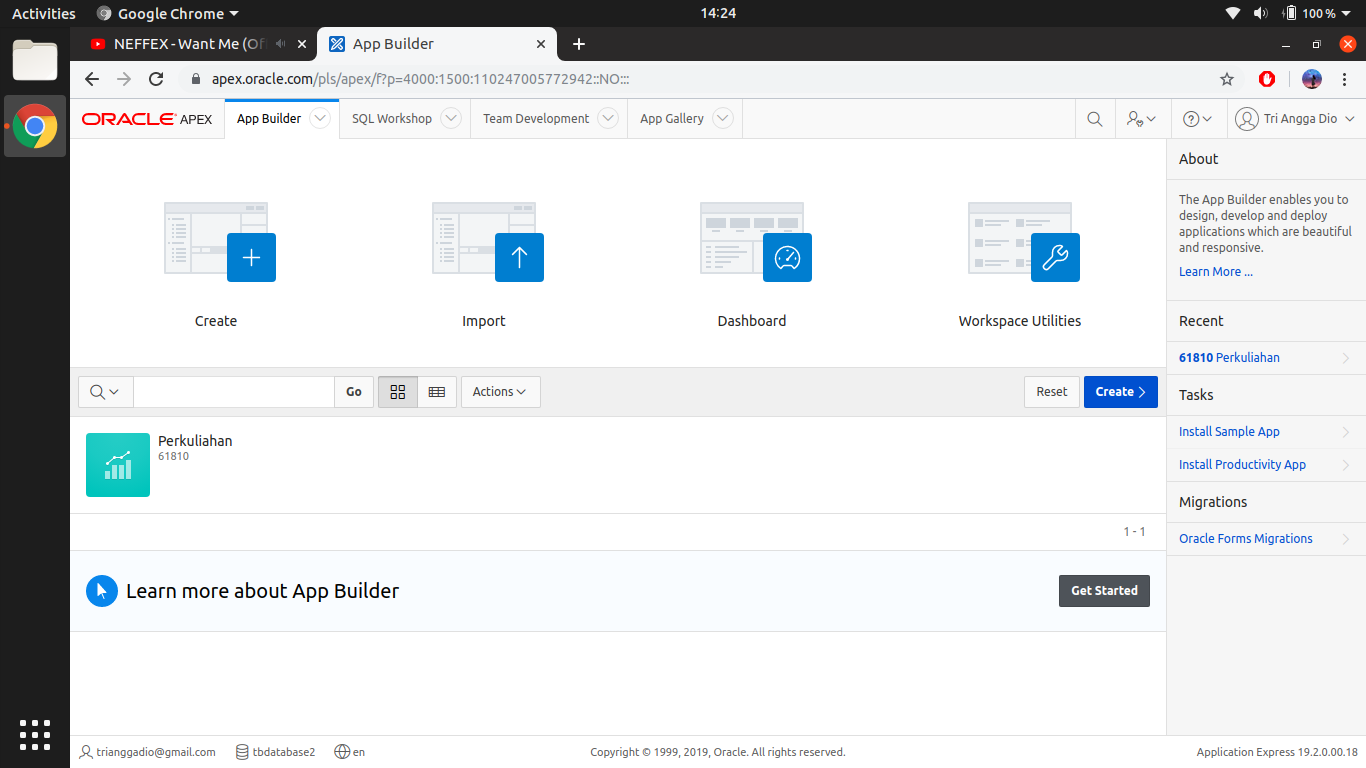
\includegraphics[width=1\textwidth]{figures/1}
\label{1}
\end{figure}

\item Setelah itu klik \textit{app builder} dan klik create hasilnya akan seperti gambar \ref{2}
\begin{figure}[H]
\centering
\caption{Halaman App Builder}
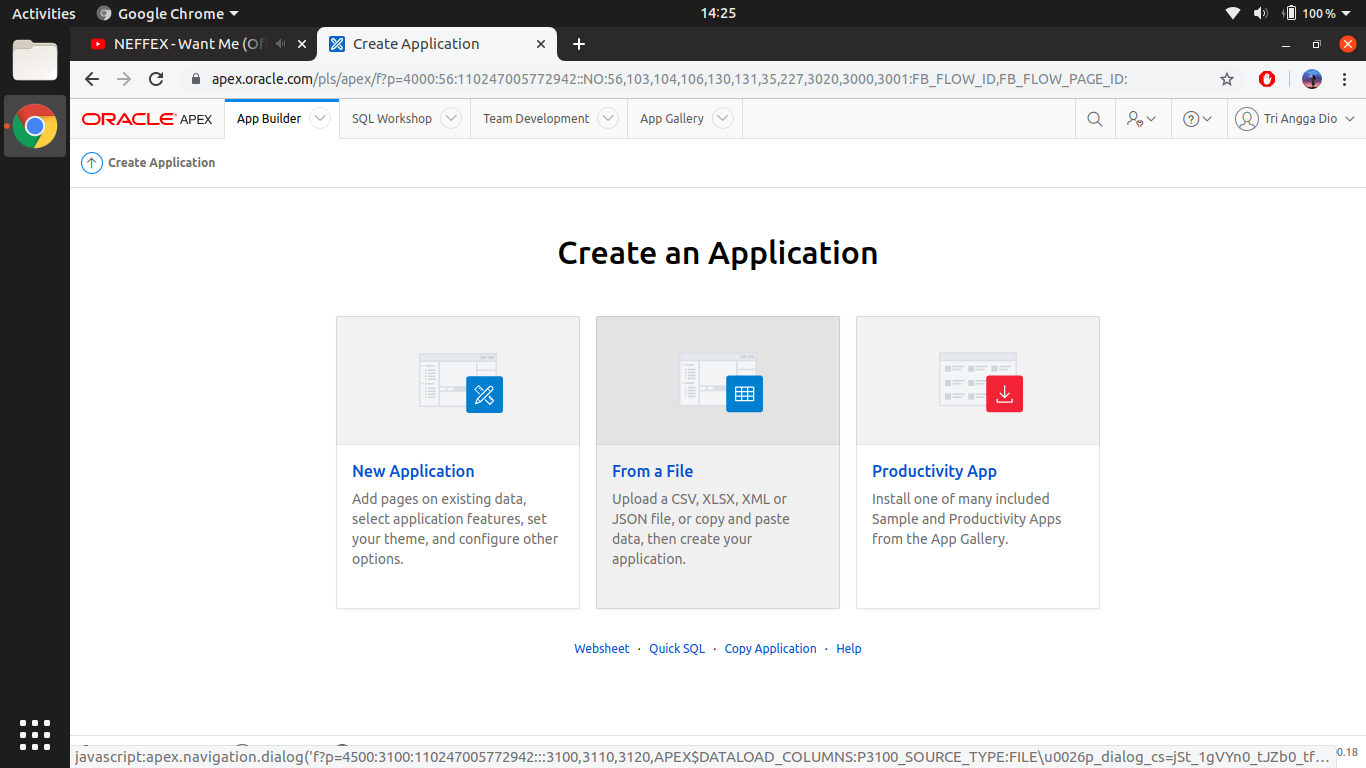
\includegraphics[width=1\textwidth]{figures/2}
\label{2}
\end{figure}

\item Selanjutnya kita, klik From a File hasilnya seperti gambar \ref{14}
\begin{figure}[H]
\centering
\caption{Halaman Upload File}
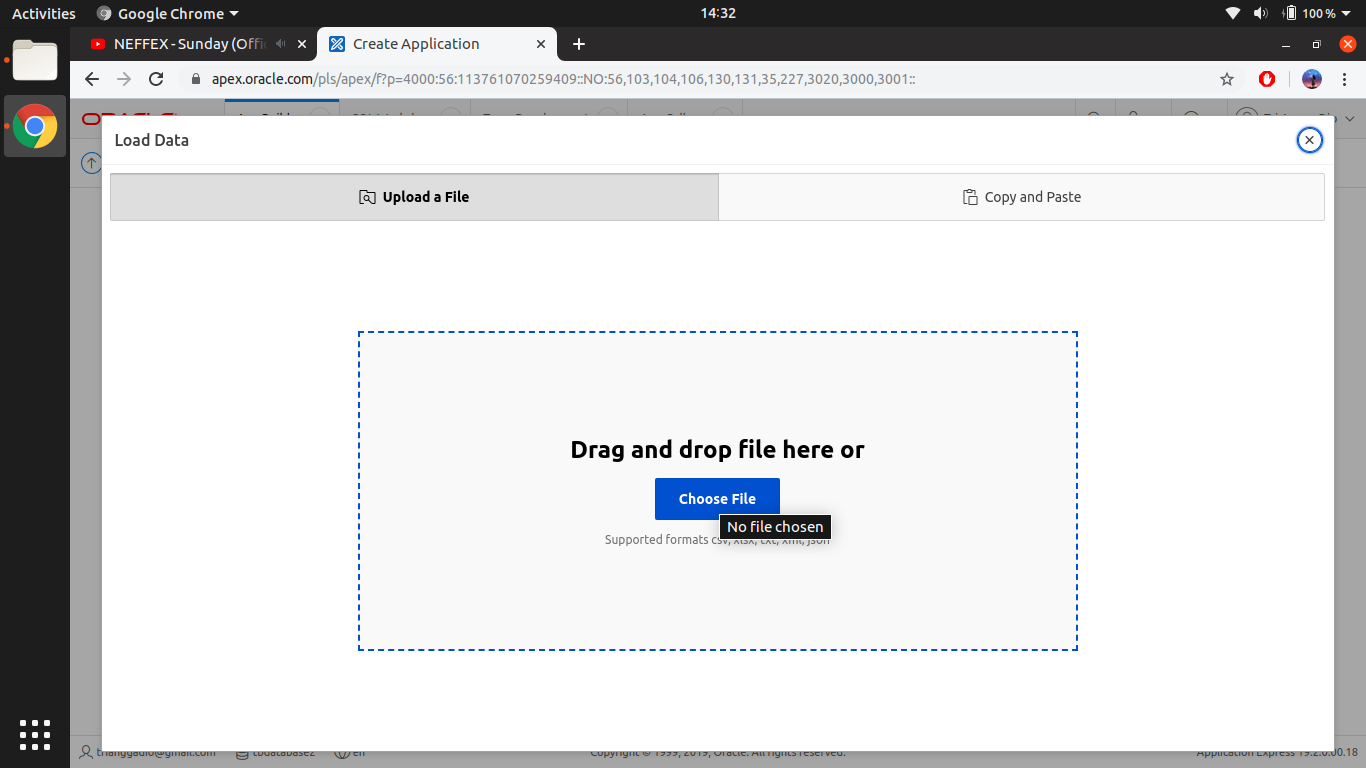
\includegraphics[width=1\textwidth]{figures/14}
\label{14}
\end{figure}

\item Setelah kita klik Choose File akan muncul window untuk memilih file xlsx atau csv seperti gambar \ref{3}
\begin{figure}[H]
\centering
\caption{Form Upload FIle}
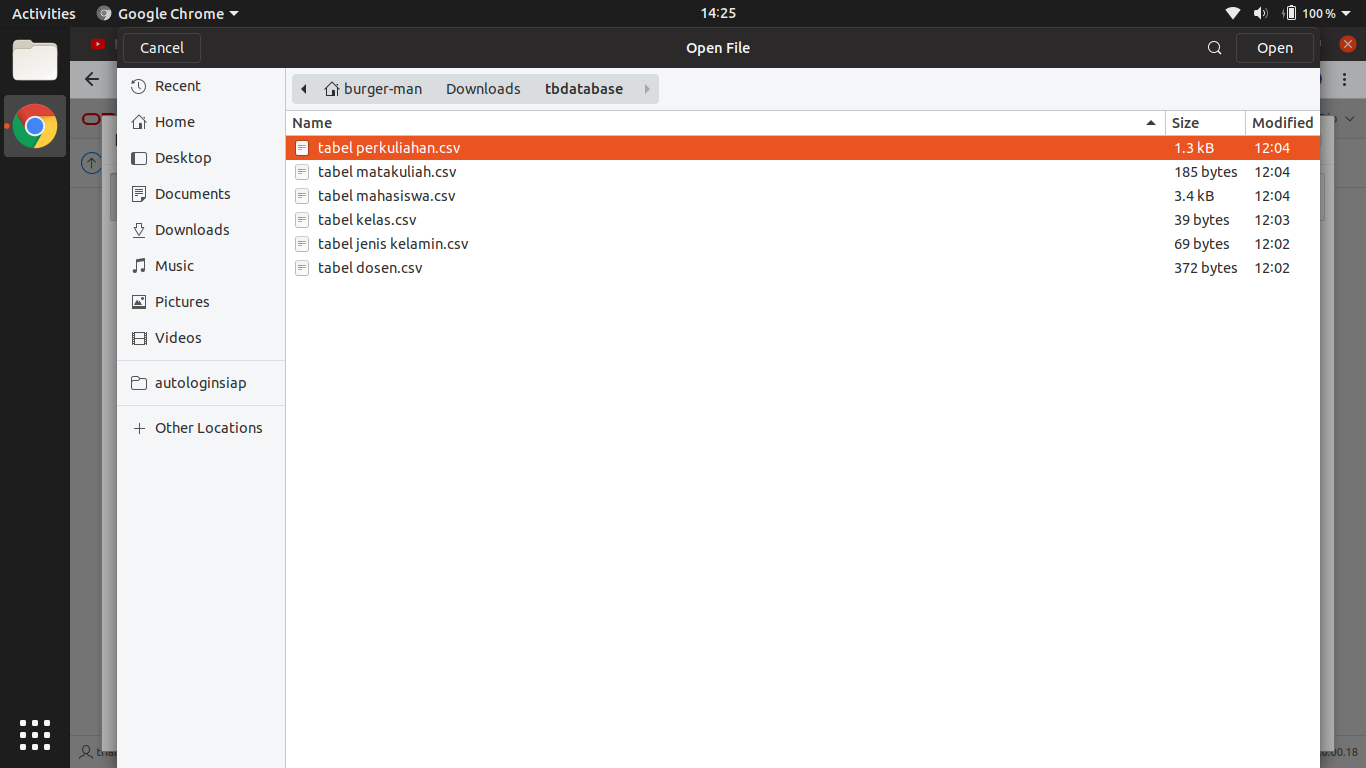
\includegraphics[width=1\textwidth]{figures/3}
\label{3}
\end{figure}

\item Setelah kita pilih dan klik open maka akan seperti gambar \ref{4}
\begin{figure}[H]
\centering
\caption{Hasil Upload File}
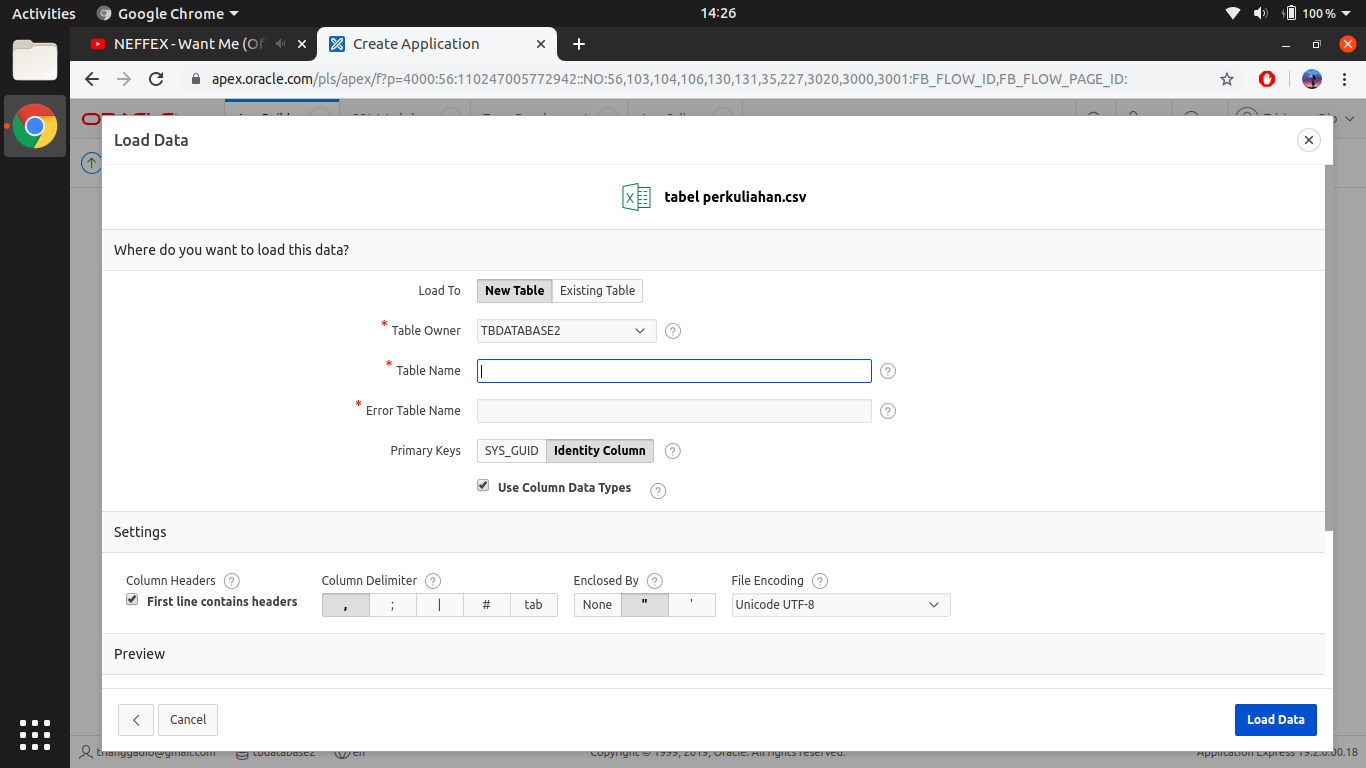
\includegraphics[width=1\textwidth]{figures/4}
\label{4}
\end{figure}

\item Setelah kita pilih selanjutnya kita masukkan nama tabelnya lalu klik field error table name hasilnya seperti gambar \ref{5}
\begin{figure}[H]
\centering
\caption{Masukkan Table Name dan Error Table Name}
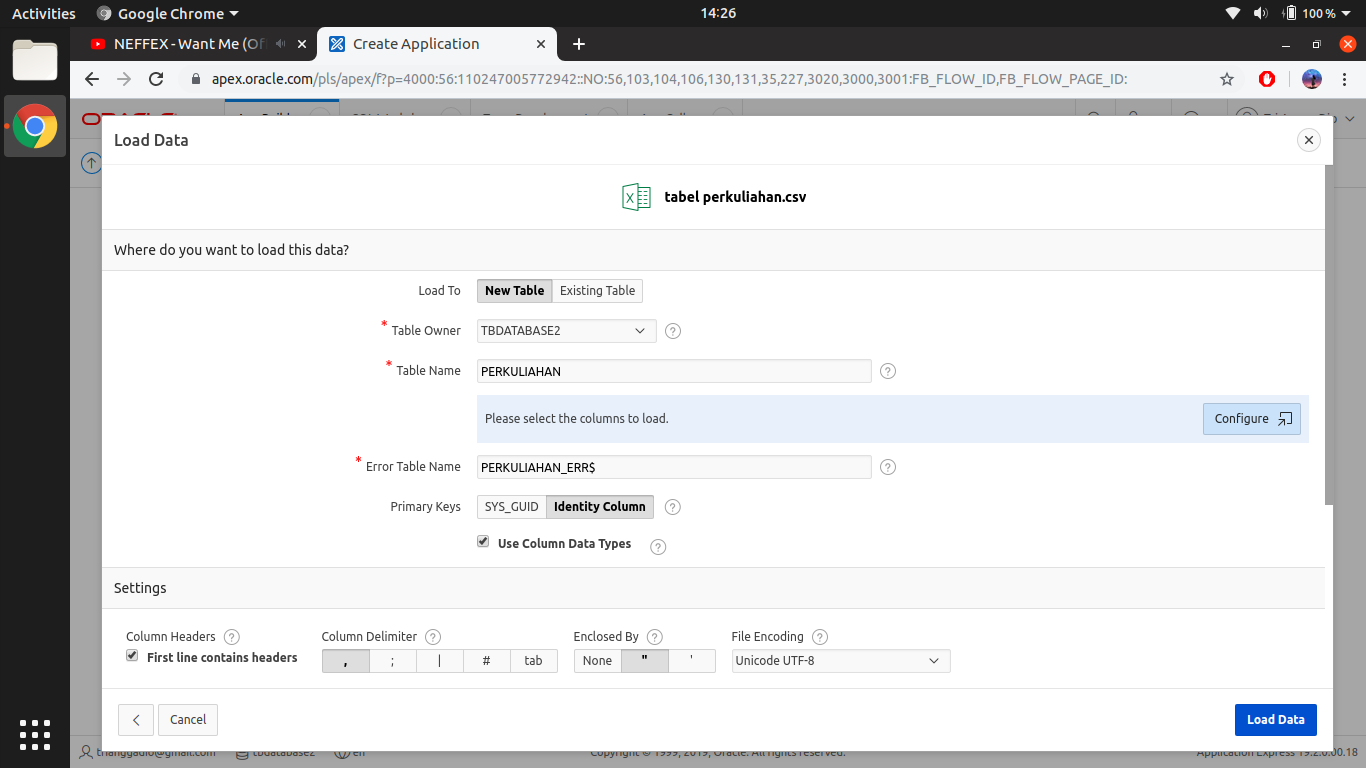
\includegraphics[width=1\textwidth]{figures/5}
\label{5}
\end{figure}

\item Klik configure untuk memastikan bahwa atribut sudah benar seperti gambar \ref{6}
\begin{figure}[H]
\centering
\caption{Configure Tabel}
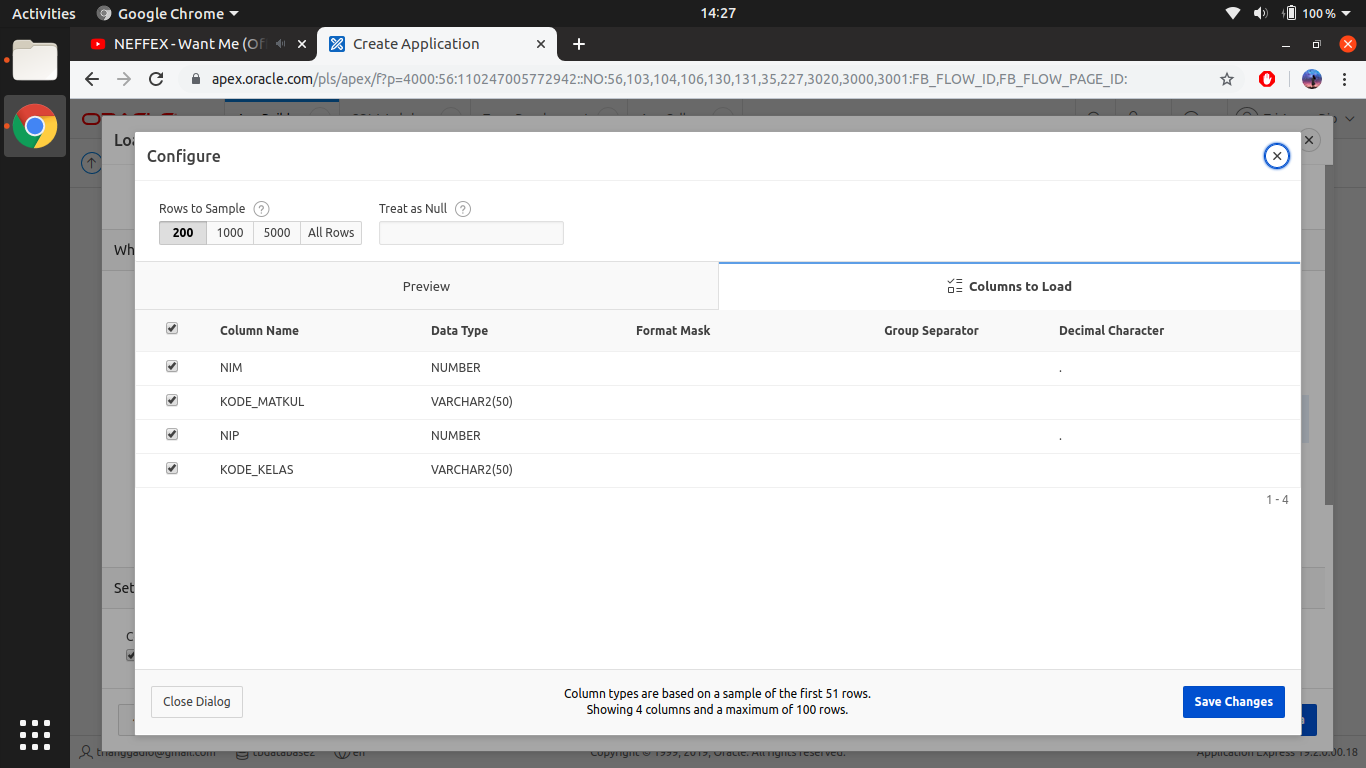
\includegraphics[width=1\textwidth]{figures/6}
\label{6}
\end{figure}

\item Setelah itu klik save change hingga hasilnya seperti gambar \ref{7}
\begin{figure}[H]
\centering
\caption{Selesai Save Change}
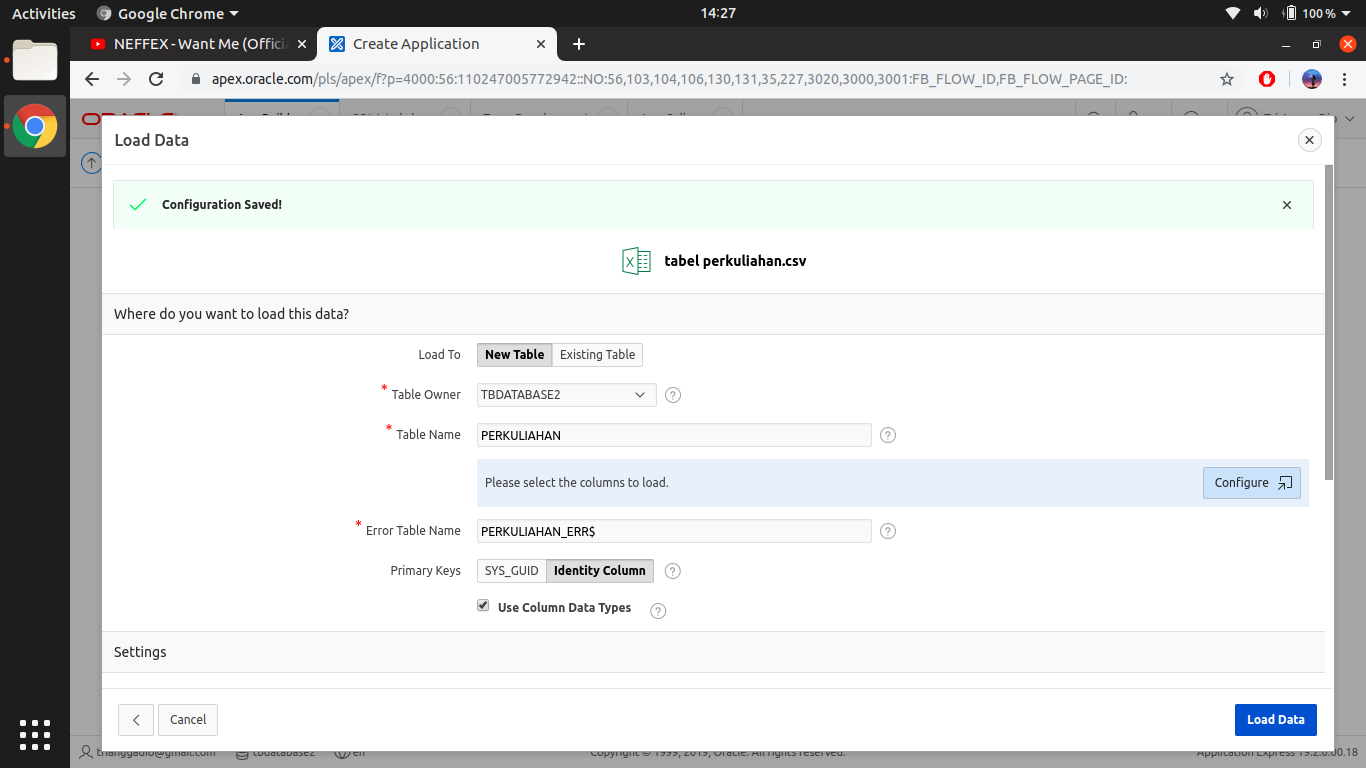
\includegraphics[width=1\textwidth]{figures/7}
\label{7}
\end{figure}

\item Lalu klik load data dan tunggu hingga berhasil seperti gambar \ref{8}
\begin{figure}[H]
\centering
\caption{Upload Selesai}
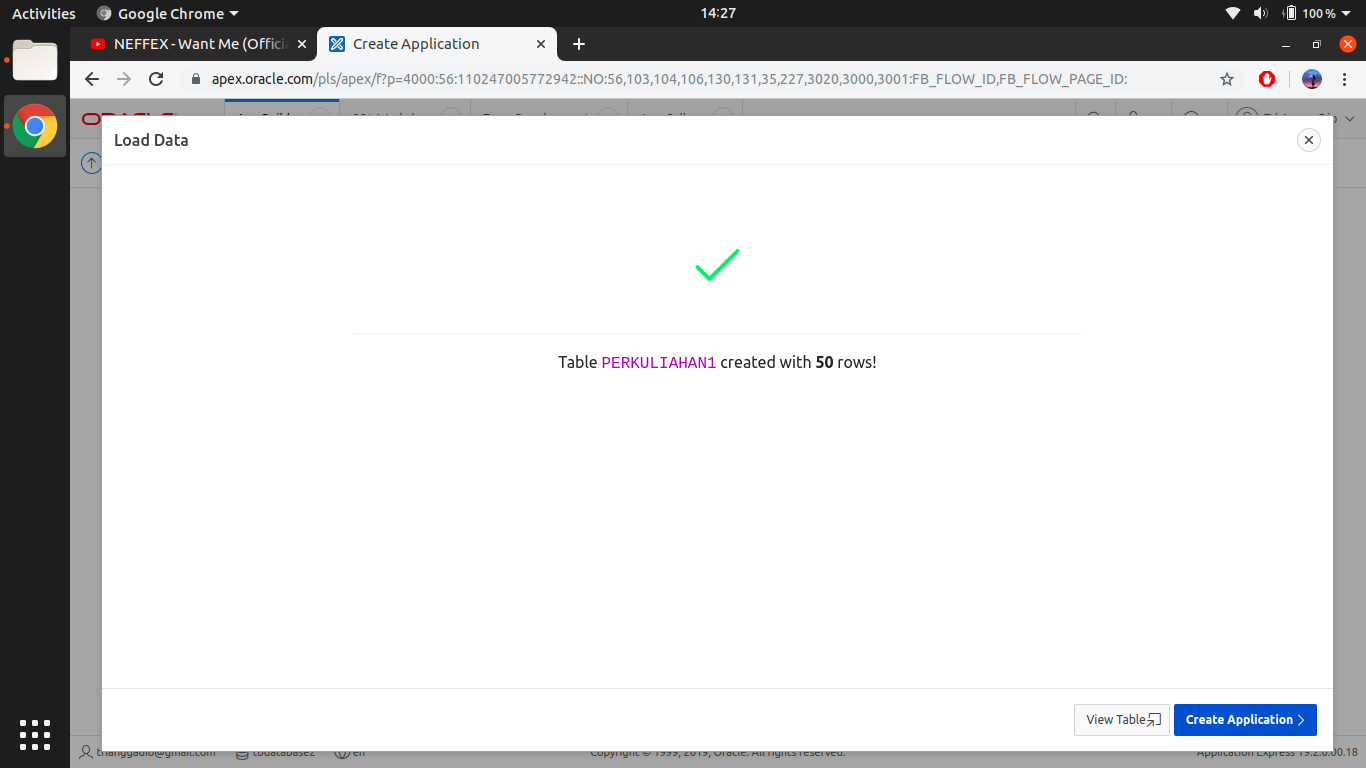
\includegraphics[width=1\textwidth]{figures/8}
\label{8}
\end{figure}

\item Lakukan berulang dari tahap 3 hingga tahap 10 sesuai tabel yang diupload

\item Jika sudah kita akan melakukan penghapusan kolom ID, ini dikarenakan ID diberikan otomatis oleh sistem apex jika di file kita tidak memiliki primary key.

\item Kita klik sql workshop lalu ke object browser
\begin{figure}[H]
\centering
\caption{SQL Workshop -> Object Browser}
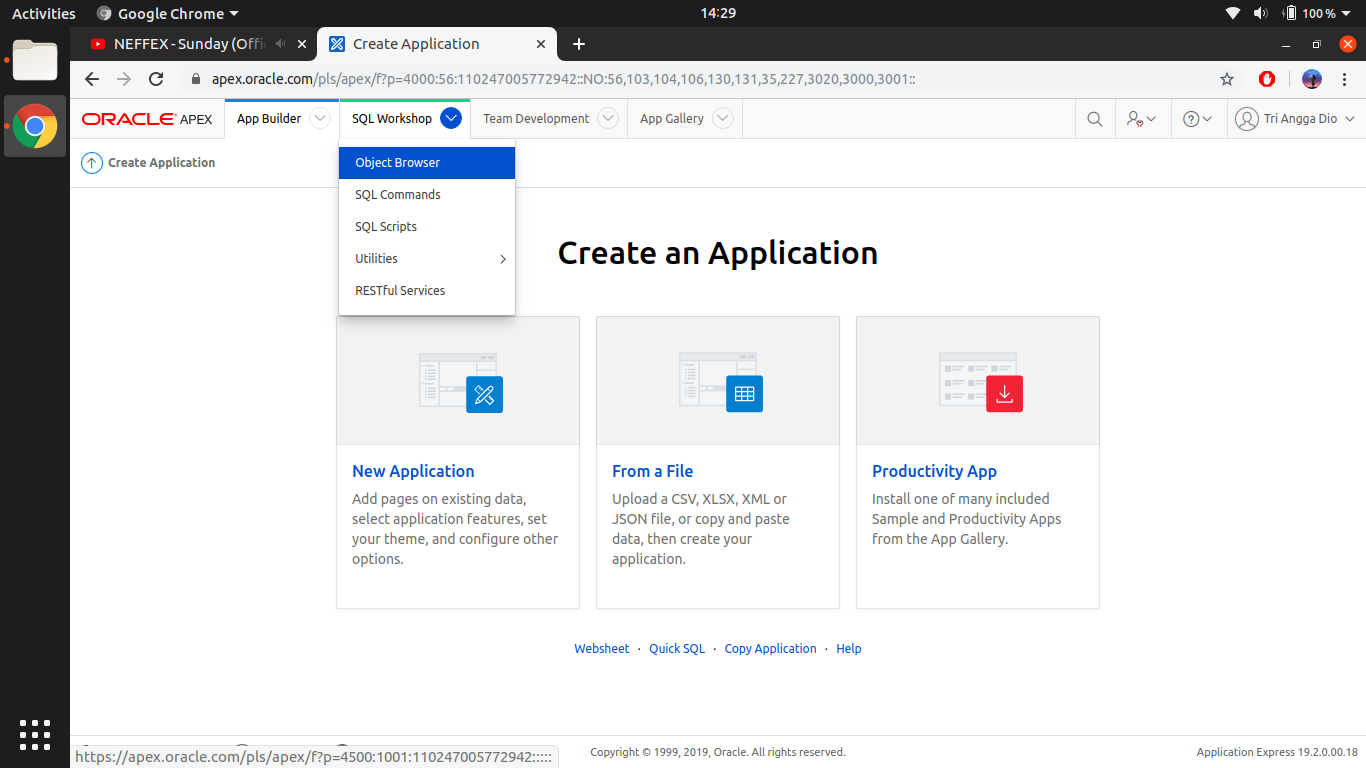
\includegraphics[width=1\textwidth]{figures/9}
\label{9}
\end{figure}

\item Selanjutnya kita klik tabel yang ingin kita drop, contohnya seperti gambar \ref{10}
\begin{figure}[H]
\centering
\caption{Tabel Drop}
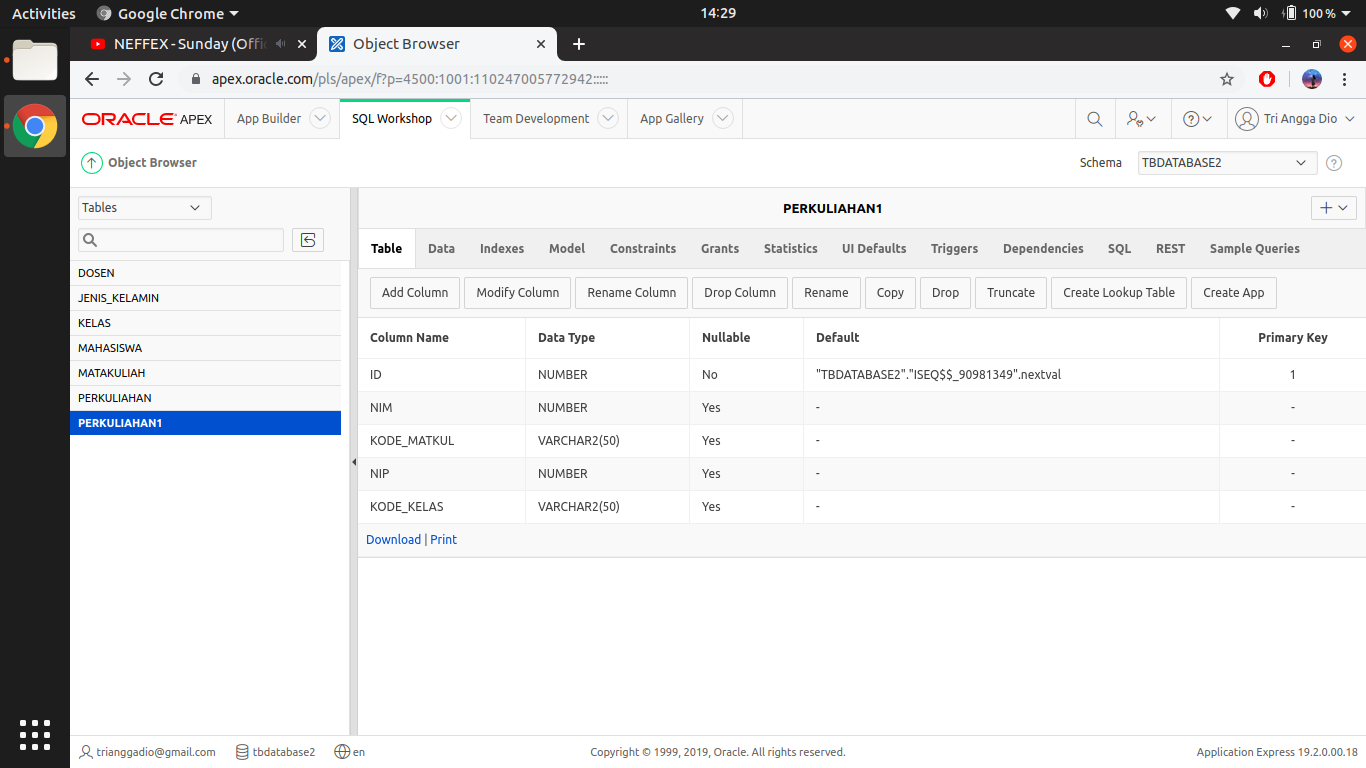
\includegraphics[width=1\textwidth]{figures/10}
\label{10}
\end{figure}

\item Jika sudah, klik Drop Column lalu pilih kolom yang ingin di drop klik drop lalu klik finish lakukan berulang hingga semua tabel terbebas dari primary key.

\item Setelah itu kita akan add primary key kesetiap tabel yang telah kita upload.

\item Lalu kita ketikkan query seperti pada gambar \ref{23}
\begin{figure}[H]
\centering
\caption{Query Add Primary Key}
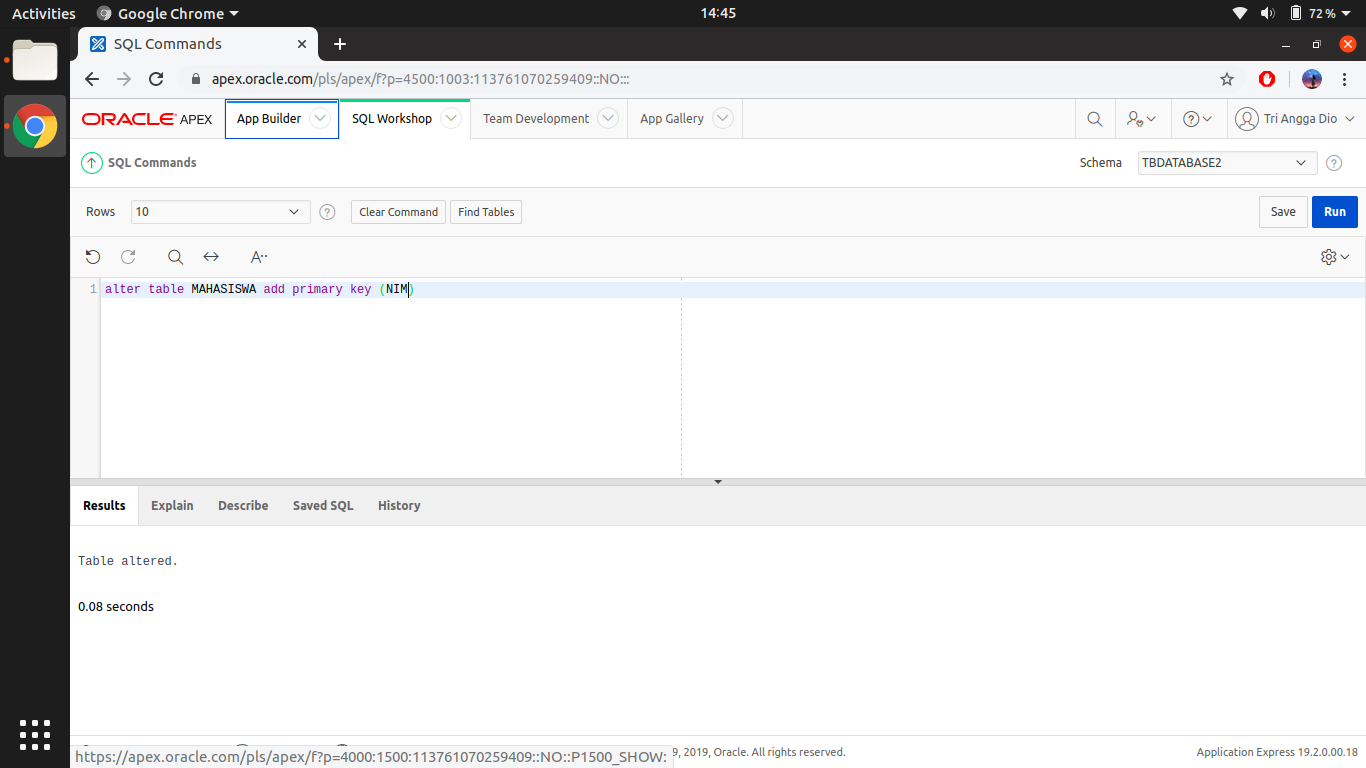
\includegraphics[width=1\textwidth]{figures/23}
\label{23}
\end{figure}

\item Setelah itu kita run, tunggu hingga muncul pesan table altered.

\item Langkah selanjutnya adalah cara merelasikan dua tabel, yaitu kita mengketikkan query seperti gambar \ref{21}
\begin{figure}[H]
\centering
\caption{Query Add Foreign Key}
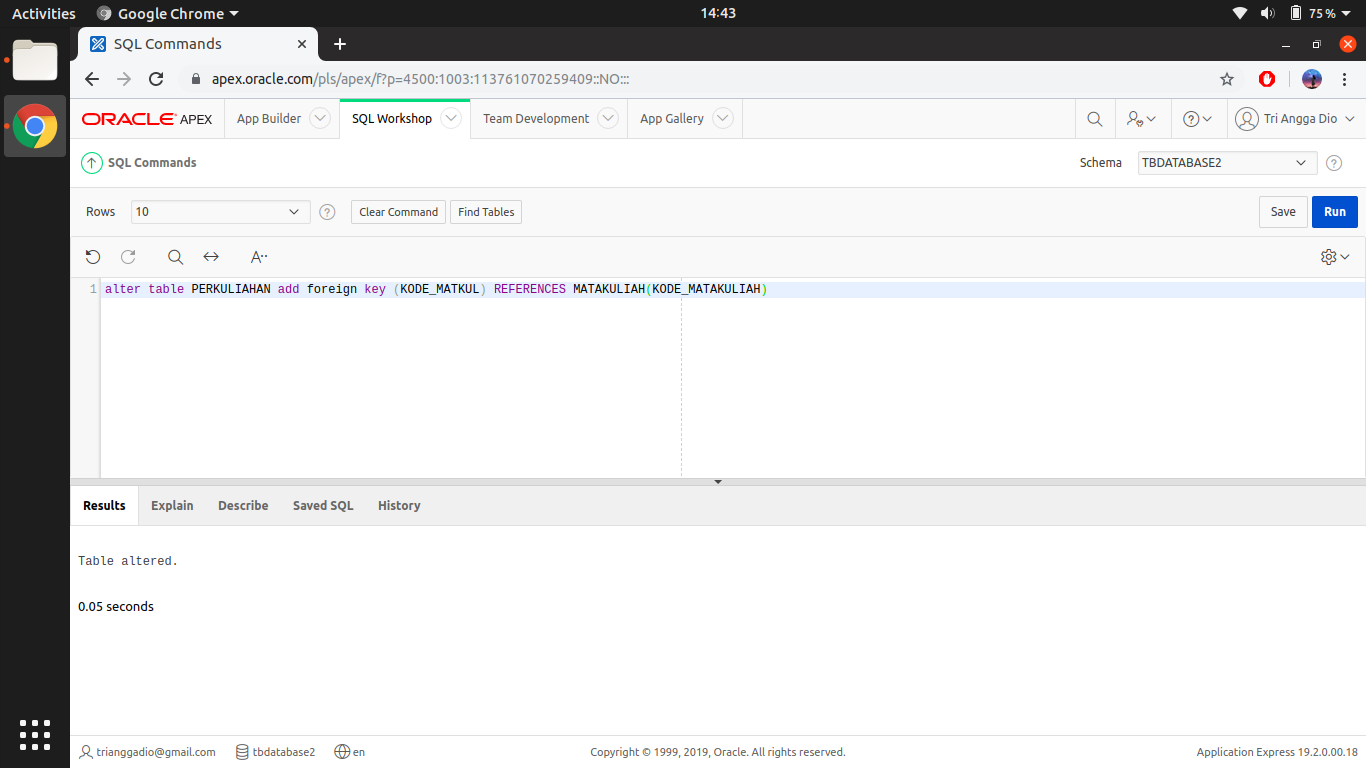
\includegraphics[width=1\textwidth]{figures/21}
\label{21}
\end{figure}

\item Langkah selanjutnya kita ke app builder lalu klik create lalu klik new application seperti gambar \ref{24}
\begin{figure}[H]
\centering
\caption{New Application}
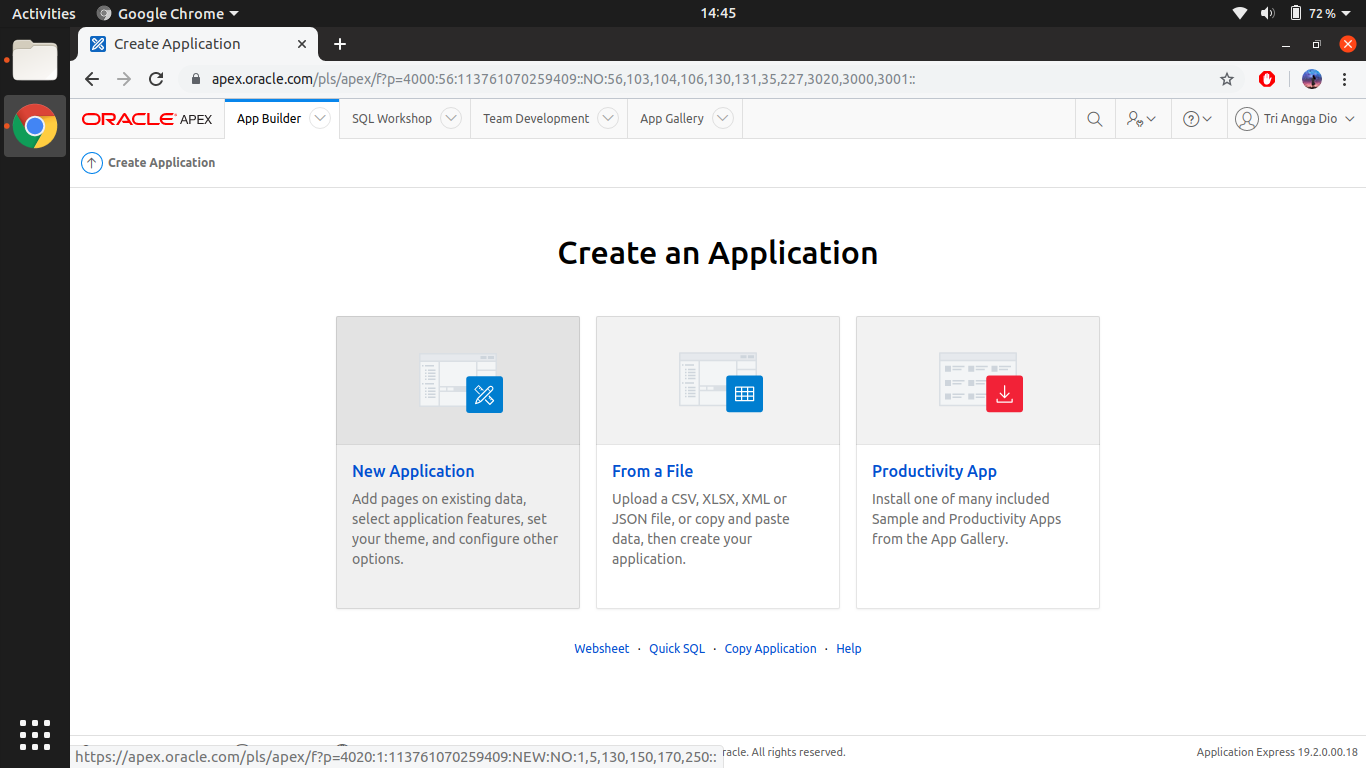
\includegraphics[width=1\textwidth]{figures/24}
\label{24}
\end{figure}

\item Setelah itu add page
\begin{figure}[H]
\centering
\caption{Add Page}
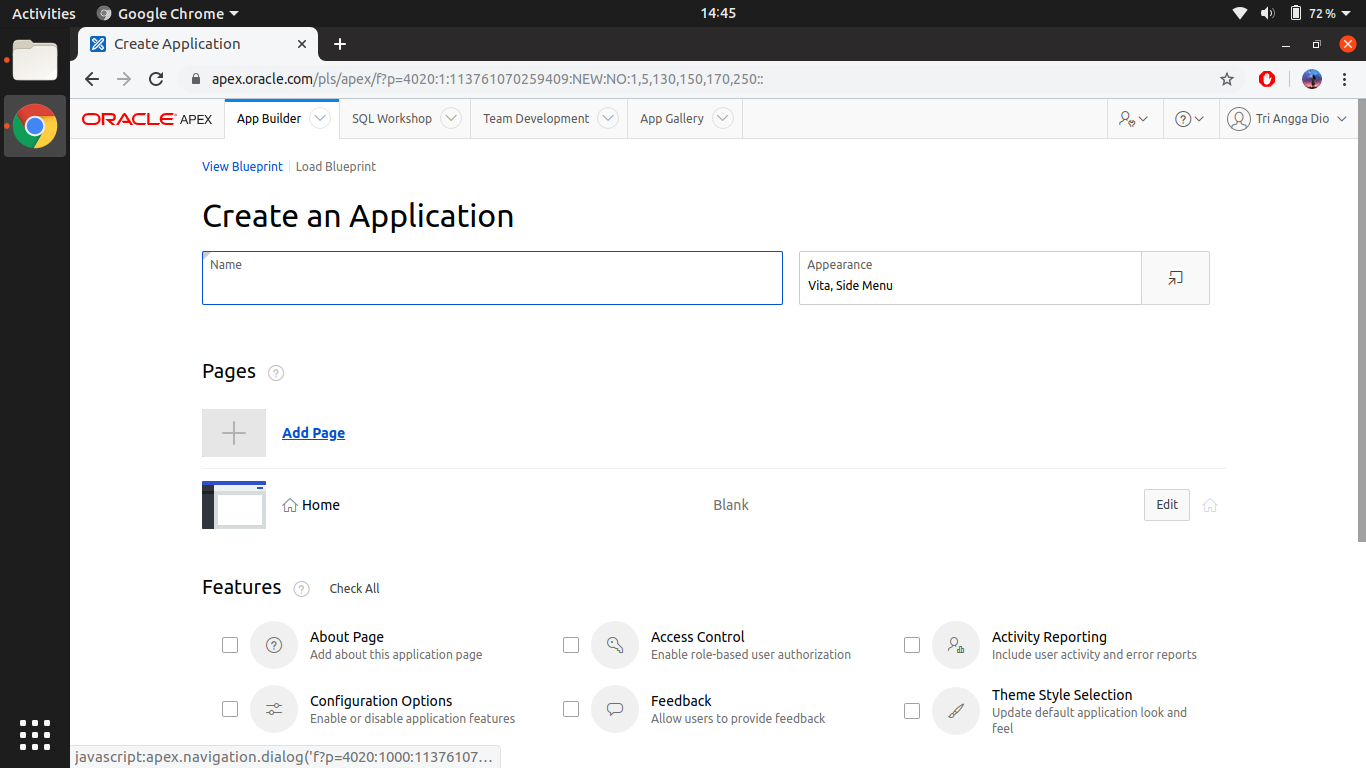
\includegraphics[width=1\textwidth]{figures/25}
\label{25}
\end{figure}

\item Kita pilih interactive report
\begin{figure}[H]
\centering
\caption{Interactive Report}
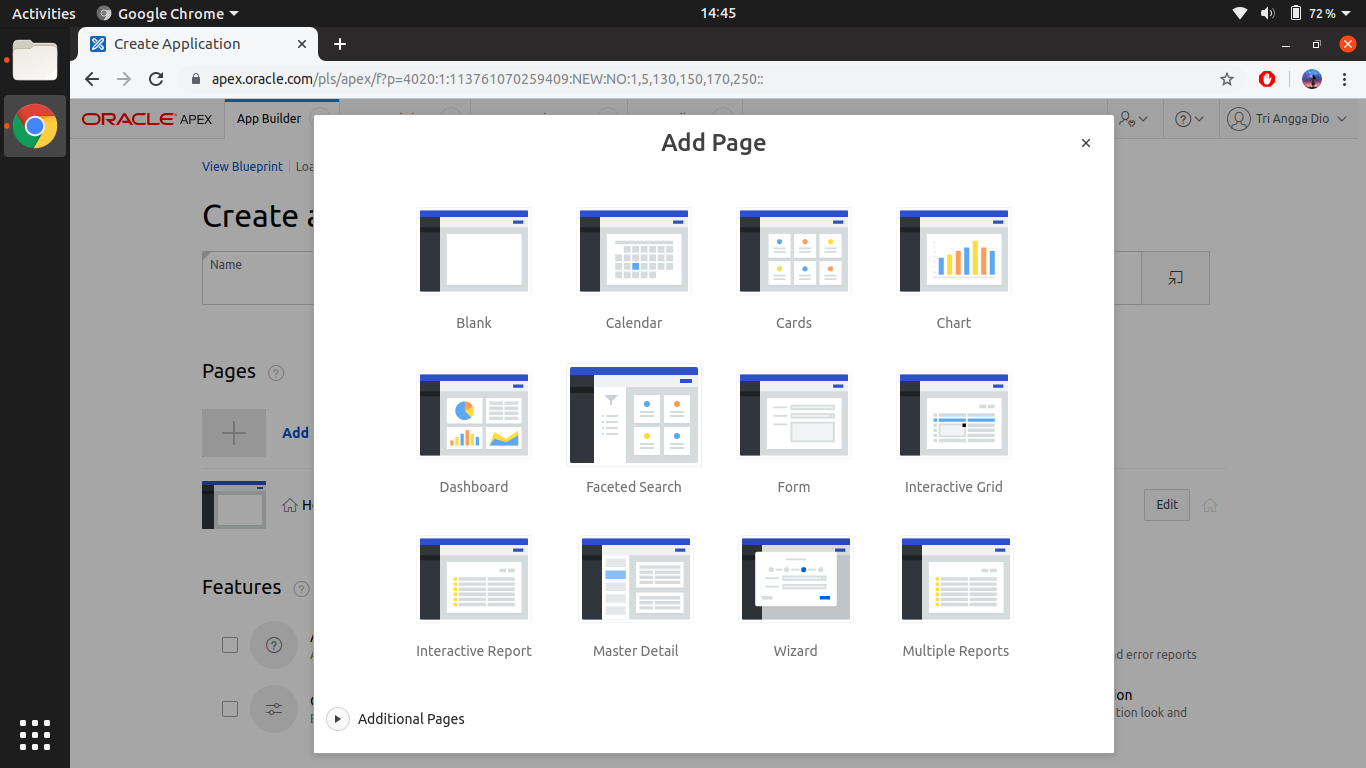
\includegraphics[width=1\textwidth]{figures/26}
\label{26}
\end{figure}

\item Lalu kita klik select table, lalu pilih tabelnya seperti gambar \ref{28}
\begin{figure}[H]
\centering
\caption{Pilih Tabel}
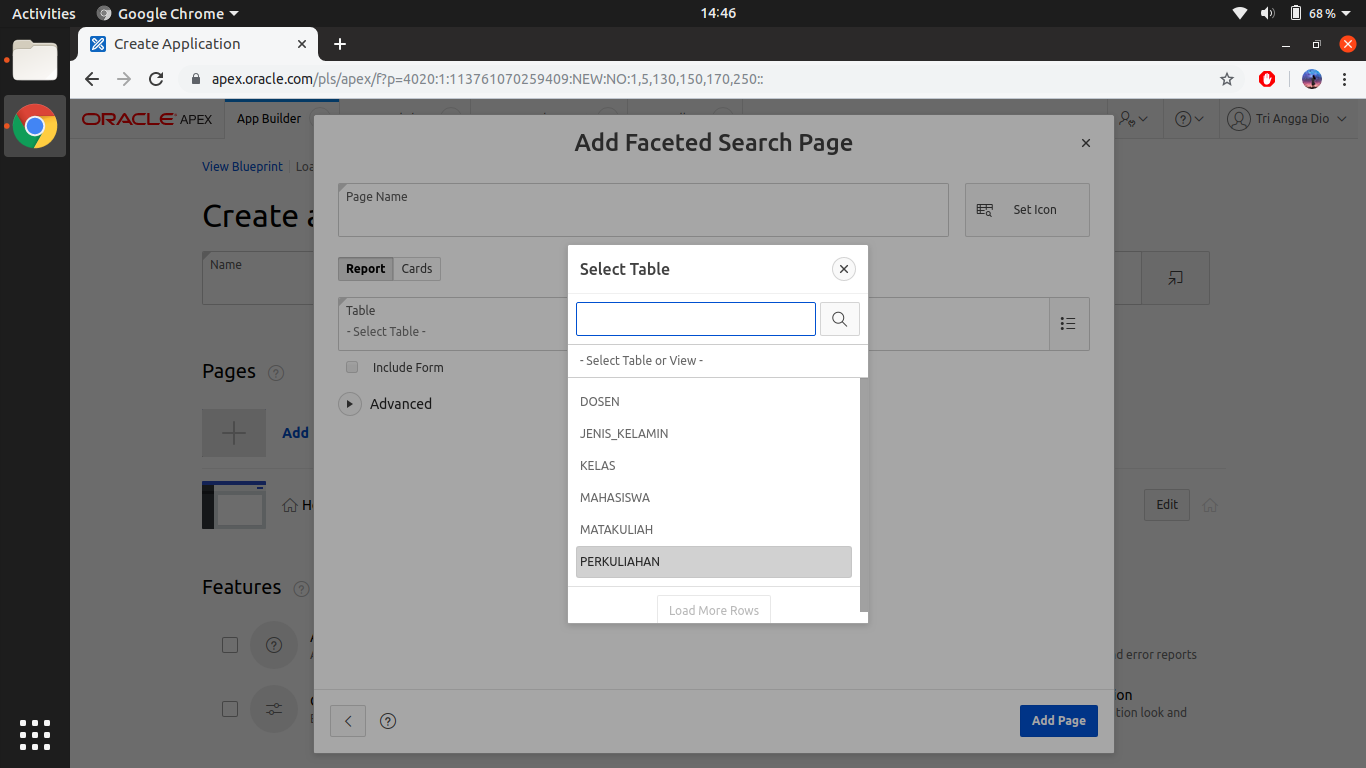
\includegraphics[width=1\textwidth]{figures/28}
\label{28}
\end{figure}

\item Setelah itu kita isi page name lalu klik ok
\begin{figure}[H]
\centering
\caption{Isi Page Name}
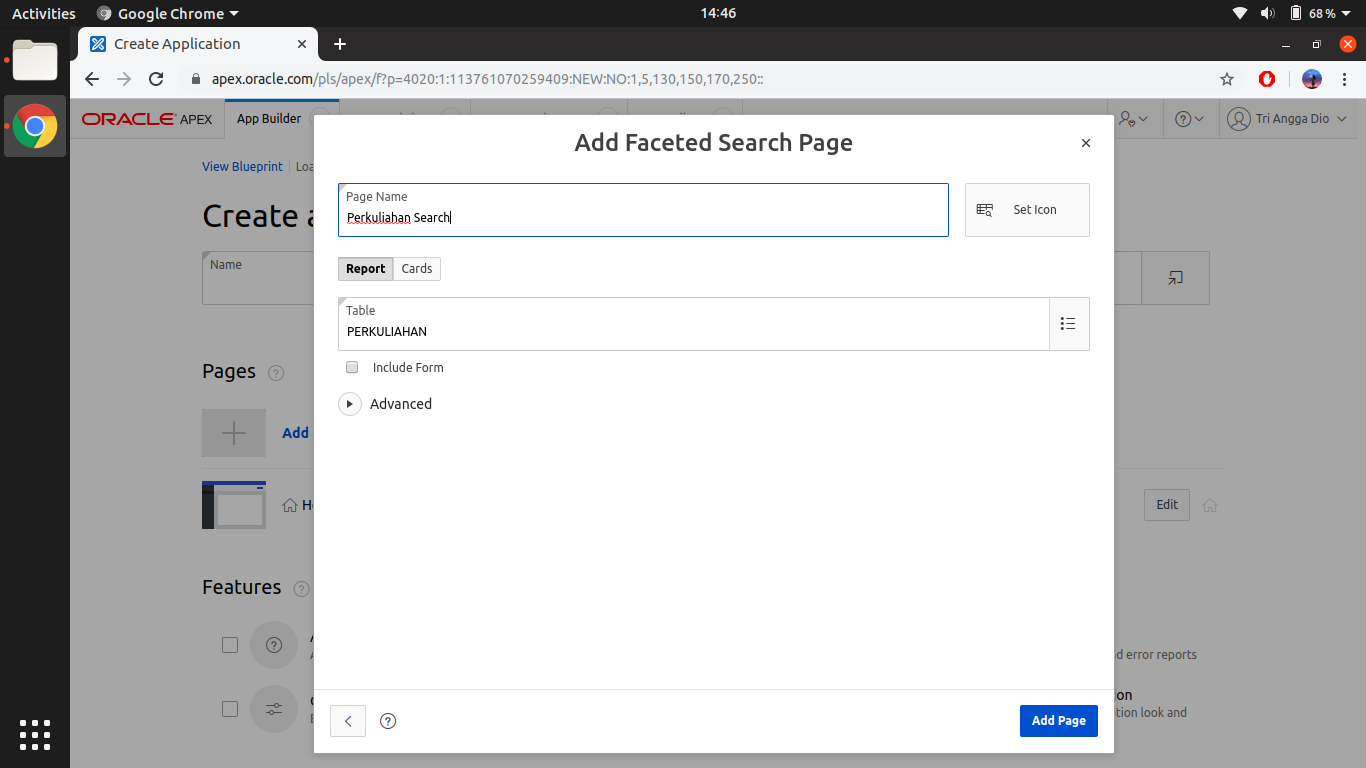
\includegraphics[width=1\textwidth]{figures/29}
\label{29}
\end{figure}

\item Ulangi step tersebut hingga sesuai kebutuhan.

\item scroll kebawah lalu klik create application

\item setelah itu kita run application seperti gambar \ref{30}
\begin{figure}[H]
\centering
\caption{Run Application}
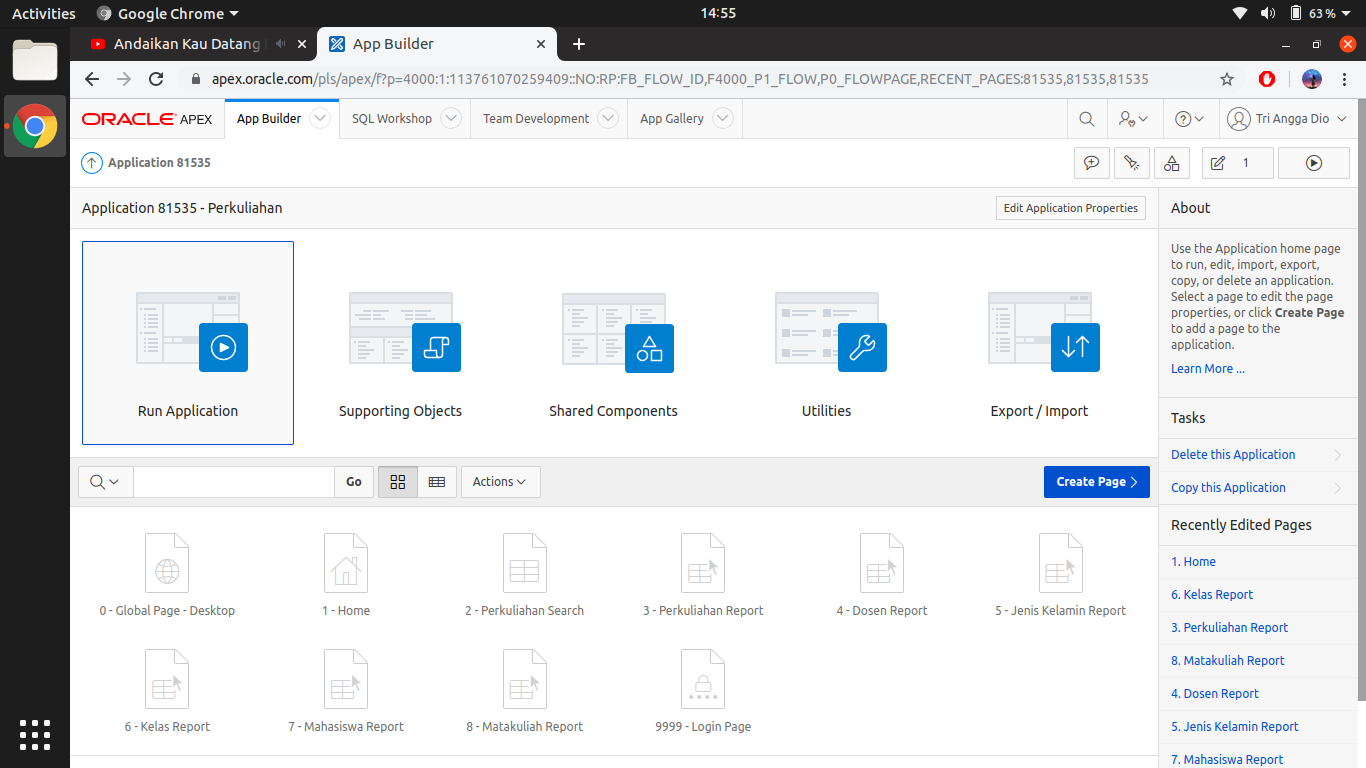
\includegraphics[width=1\textwidth]{figures/31}
\label{31}
\end{figure}

\item Hasilnya seperti gambar \ref{32} dan gambar \ref{33}
\begin{figure}[H]
\centering
\caption{Hasil 2}
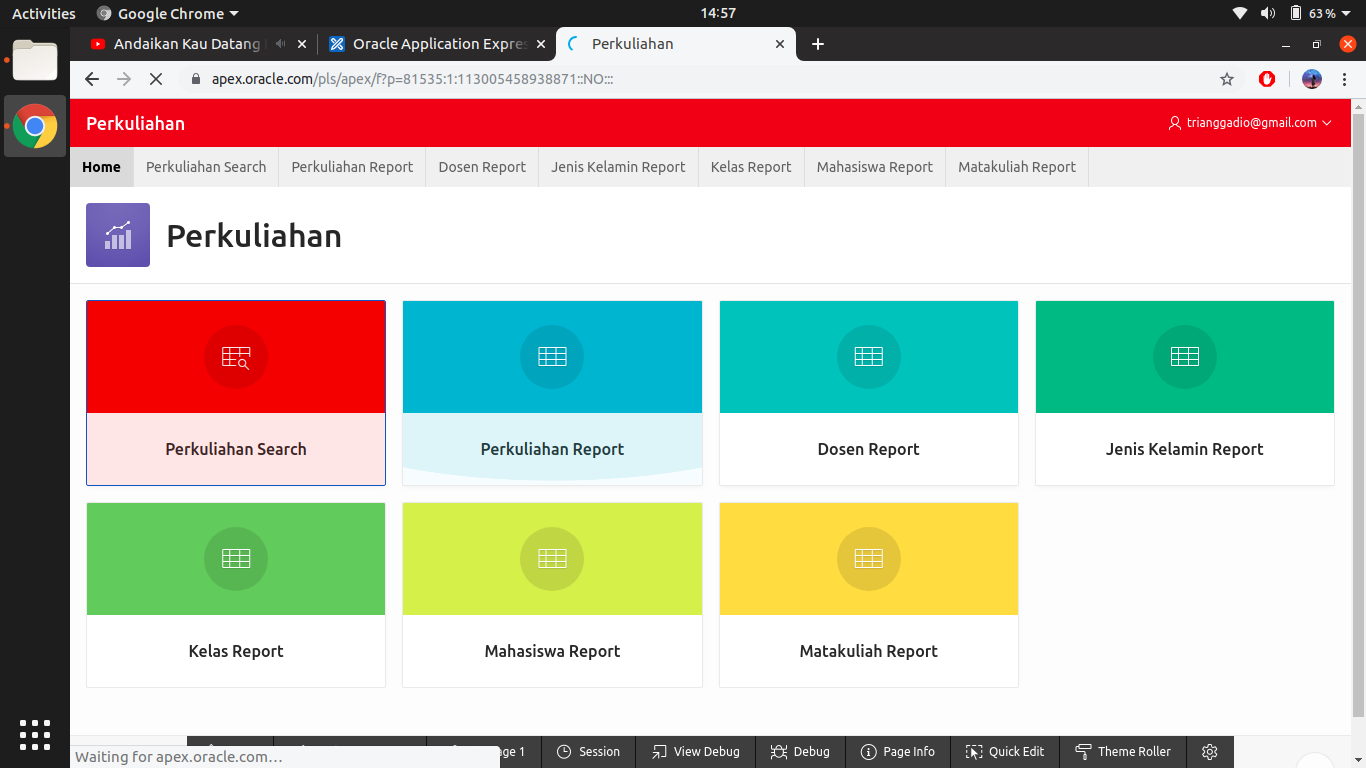
\includegraphics[width=1\textwidth]{figures/32}
\label{32}
\end{figure}

\begin{figure}[H]
\centering
\caption{Hasil 2}
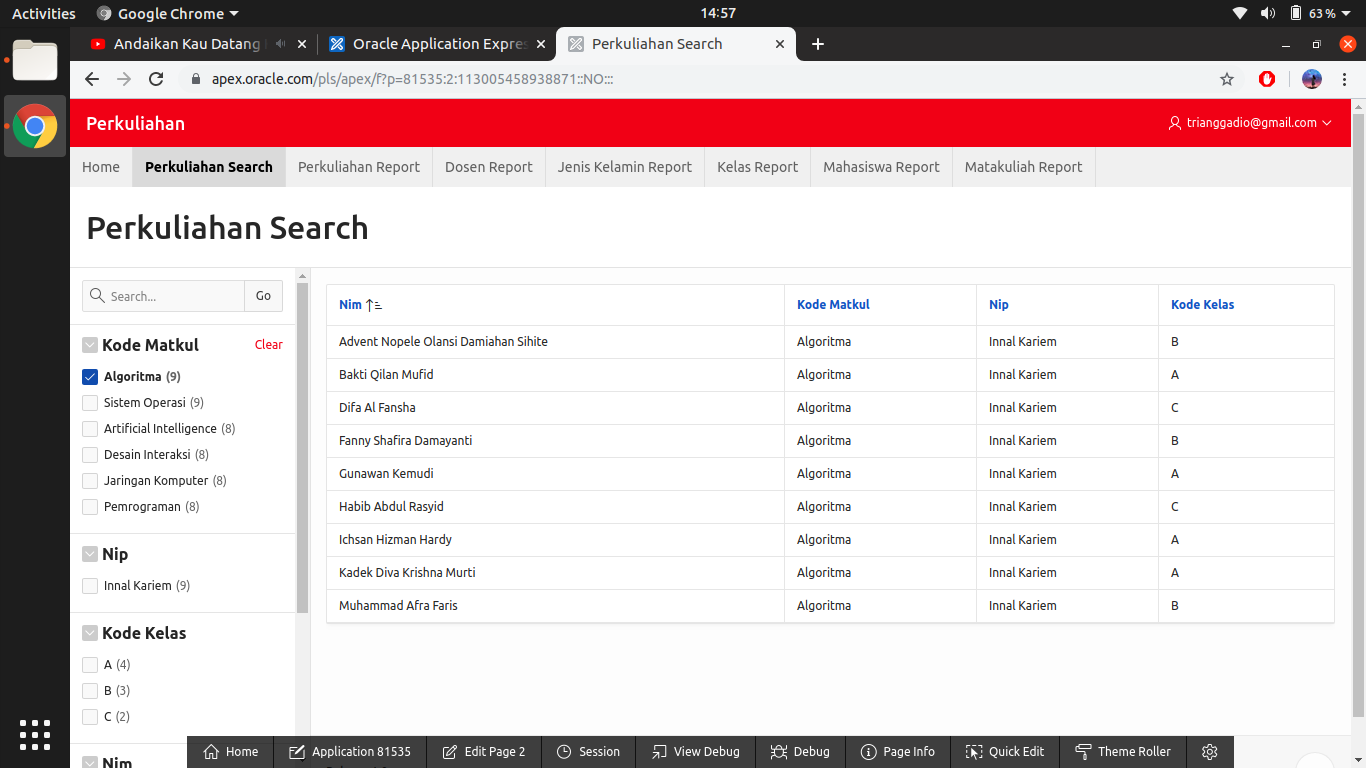
\includegraphics[width=1\textwidth]{figures/33}
\label{33}
\end{figure}

\end{enumerate}